\documentclass[12pt, a4paper]{article}
\usepackage[left=2cm,right=2cm, top=2cm,bottom=2cm,bindingoffset=0cm]{geometry}
\usepackage[utf8]{inputenc}
\usepackage{indentfirst}
\usepackage[russian]{babel}
\usepackage{amssymb}
\usepackage{xcolor}
\usepackage{hyperref}
\usepackage{indentfirst}
\usepackage{ upgreek }
\usepackage[document]{ragged2e}
\usepackage{graphicx}
\usepackage{wrapfig}
\definecolor{linkcolor}{HTML}{00BFFF} % цвет ссылок
\definecolor{urlcolor}{HTML}{00BFFF} % цвет гиперссылок
 
\hypersetup{pdfstartview=FitH,  linkcolor=linkcolor,urlcolor=urlcolor, colorlinks=true}

\graphicspath{ {./images/} }

\newcommand{\Expect}{\mathbb{E}}

\title{SDP релаксация для задачи поиска максимального разреза}
\author{Роман Горб}
\date{Декабрь 2019}

\begin{document}

\maketitle

\begin{abstract}
Темой данного курсового проекта является решение NP-полной задачи Max Сut. Начиная с приведения постановки задачи, речь пойдет о построении релаксации в терминах полуопределенного программирования(SDP), затем будет описан и доказан алгоритм Гёманса–Уильямсона восстановления разреза, и, наконец, будет произведен анализ работы его реализации на различных классических наборах тестов.
\end{abstract}

\tableofcontents

\newpage

\section{Постановка задачи}

\begin{wrapfigure}{r}{0.25\textwidth}
    \centering
    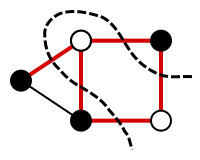
\includegraphics[width=0.25\textwidth]{images/Max-cut.png}
    \caption{\\Пример разреза\\(ребра, пересекающие разрез, выделены красным)}
    \label{fig:fig1}
\end{wrapfigure}

Дан неориентированный граф $G(V, E)$ с матрицей весов $W \in S^n$, $W \geqslant 0$. Требуется построить такое разбиение множества вершин $V=S\sqcup T$, что суммарный вес ребер, ведущих из $S$ в $T$, был \textbf{максимально} возможным. Иначе говоря, нужно решить следующую задачу оптимизации:
$$c^* = \max \limits_{x} \frac{1}{4} \sum_{i = 1}^{n} \sum_{j = 1}^{n} w_{ij}(1 - x_i x_j)$$
$$s.t.\: x_i =\pm1$$

\section{Построение SDP задачи}
Поставленные в задаче бинарные ограничения делают ее задачей дискретной оптимизации. Переформулируем задачу к виду проверки на существование в графе $G$ разреза стоимостью хотя бы $k$. Эта задача лежит в NP, потому что в качестве сертификата в данном случае можно использовать разрез. Можно доказать сводимость к ней задачи 3-SAT(что хорошо описано, например, у David Steurer\cite{reduction}), что уже влечет ее NP-полноту. Поэтому имеет смысл построения более простой задачи, которая вычислялась бы за разумное время.

Пусть матрица $Y=xx^T$, тогда $x_i x_j = y_{ij}$. Значит ограничение $x_i = \pm 1$ есть тоже самое, что $diag(Y) = (1, \dots, 1)^T$. Заметим, что эти преобразования не поменяли суть задачи, но уже привели ее к следующему виду:
$$\max \limits_{x} \frac{1}{4} \sum_{i = 1}^{n} \sum_{j = 1}^{n} w_{ij}(1 - y_{ij})$$
$$s.t.\: Y = xx^T$$
$$diag(Y) = (1, \dots, 1)^T$$
Видим, что матрица $Y$ должна быть одноранговой. Такое ограничение делает задачу невыпуклой, поэтому предлагается избавится от него, заменив его на $Y \in S^n_+$(именно в этом моменте мы делаем не равносильное преобразование и получаем релаксацию). Избавившись от переменной $x$, получаем следующую задачу:
$$\max \limits_{Y} \frac{1}{4} \sum_{i = 1}^{n} \sum_{j = 1}^{n} w_{ij}(1 - y_{ij})$$
$$s.t.\: Y \in S_+^n$$
$$diag(Y) = (1, \dots, 1)^T$$
Убрав слагаемые, которые не зависят от $Y$, и значок транспонирования у матрицы $Y$(из симметричности) получаем следующую эквивалентную задачу:
$$\min \limits_{Y} \frac{1}{4} trace(WY)$$
$$s.t.\: Y \in S_+^n$$
$$diag(Y) = (1, \dots, 1)^T$$
Стандартная форма задачи полуопределенного программирования выглядит следующим образом:
$$\min \limits_{X} trace(CX)$$
$$s.t.\: trace(A_i X) = b_i$$
$$X \in S_+^n$$
$$C, A_i \in S^n$$
Значит единственное, что осталось, это разобраться с ограничением на след, что делается просто:
$Y_{ii} = trace(Y E^i)$, где у матрицы $E^i$ все элементы равны $0$, кроме $E^i_{ii} = 1$. Значит заменяем ограничение на диагональ $Y$ серией из $n$ ограничений $trace(Y E^i) = 1$. Итого, полученная задача \textbf{удовлетворяет стандартной форме SDP}.

\section{Алгоритм Гёманса–Уильямсона}
Когда мы решим релаксированную задачу, мы получим какую-то матрицу $X \in S^n_+$, которая все еще не является ответом(ее элементы могут быть даже не целыми). Поэтому далее будет описан алгоритм, справляющийся с этой трудностью.
\subsection{Описание}
Так матрица $Y$ симметрична и положительно полуопределена, то у нее есть спектральное разложение $Y = LDL^T$, где $D$ -- диагональная матрица, где на диагонали стоят собственные значения. Тогда $Y = UU^T$, где $U = L\sqrt{D}$.\\

Повторим следующую процедуру много раз и из ответов выберем лучший:
\begin{enumerate}
    \item
    Сгенерируем случаный вектор $v$ на единичной сфере(это можно сделать например отнормировав гауссовский вектор).
    \item
    Возмьмем за множество $S = \{i|\langle v, u_i \rangle \geqslant 0 \}$, где $u_i$ -- столбец матрицы $U$(проще говоря, возьмем те индексы, для которых соответствующие собственные вектора попали в одно полупространство при сечении гиперплоскотью с вектором нормали $v$).
\end{enumerate}

\subsection{Корректность}
\textbf{Утверждение:}

Обозначим $r^*$ -- возвращаемое алгоритмом значение(после одной итерации). Тогда
$$ c^* \geqslant \Expect_v (r^*) \geqslant 0.878 p^*$$

\textbf{Доказательство:}
Рассмотрим матожидание величины разреза, который нам вернул алгоритм(распишем по определению):
$$ \Expect_v (C) = \Expect_v \frac{1}{2} \left( \sum_{i = 1}^{n} \sum_{j=1}^{n} w_{ij} \mathrm{I}[sign(v^Tu_i) \ne sign(v^Tu_j)] \right)$$
$$ = \Expect_v \frac{1}{2} \left( \sum_{i = 1}^{n} \sum_{j=1}^{n} w_{ij} \mathbb{P}(sign(v^Tu_i) \ne sign(v^Tu_j)) \right)$$

\begin{figure}[h]
\centering
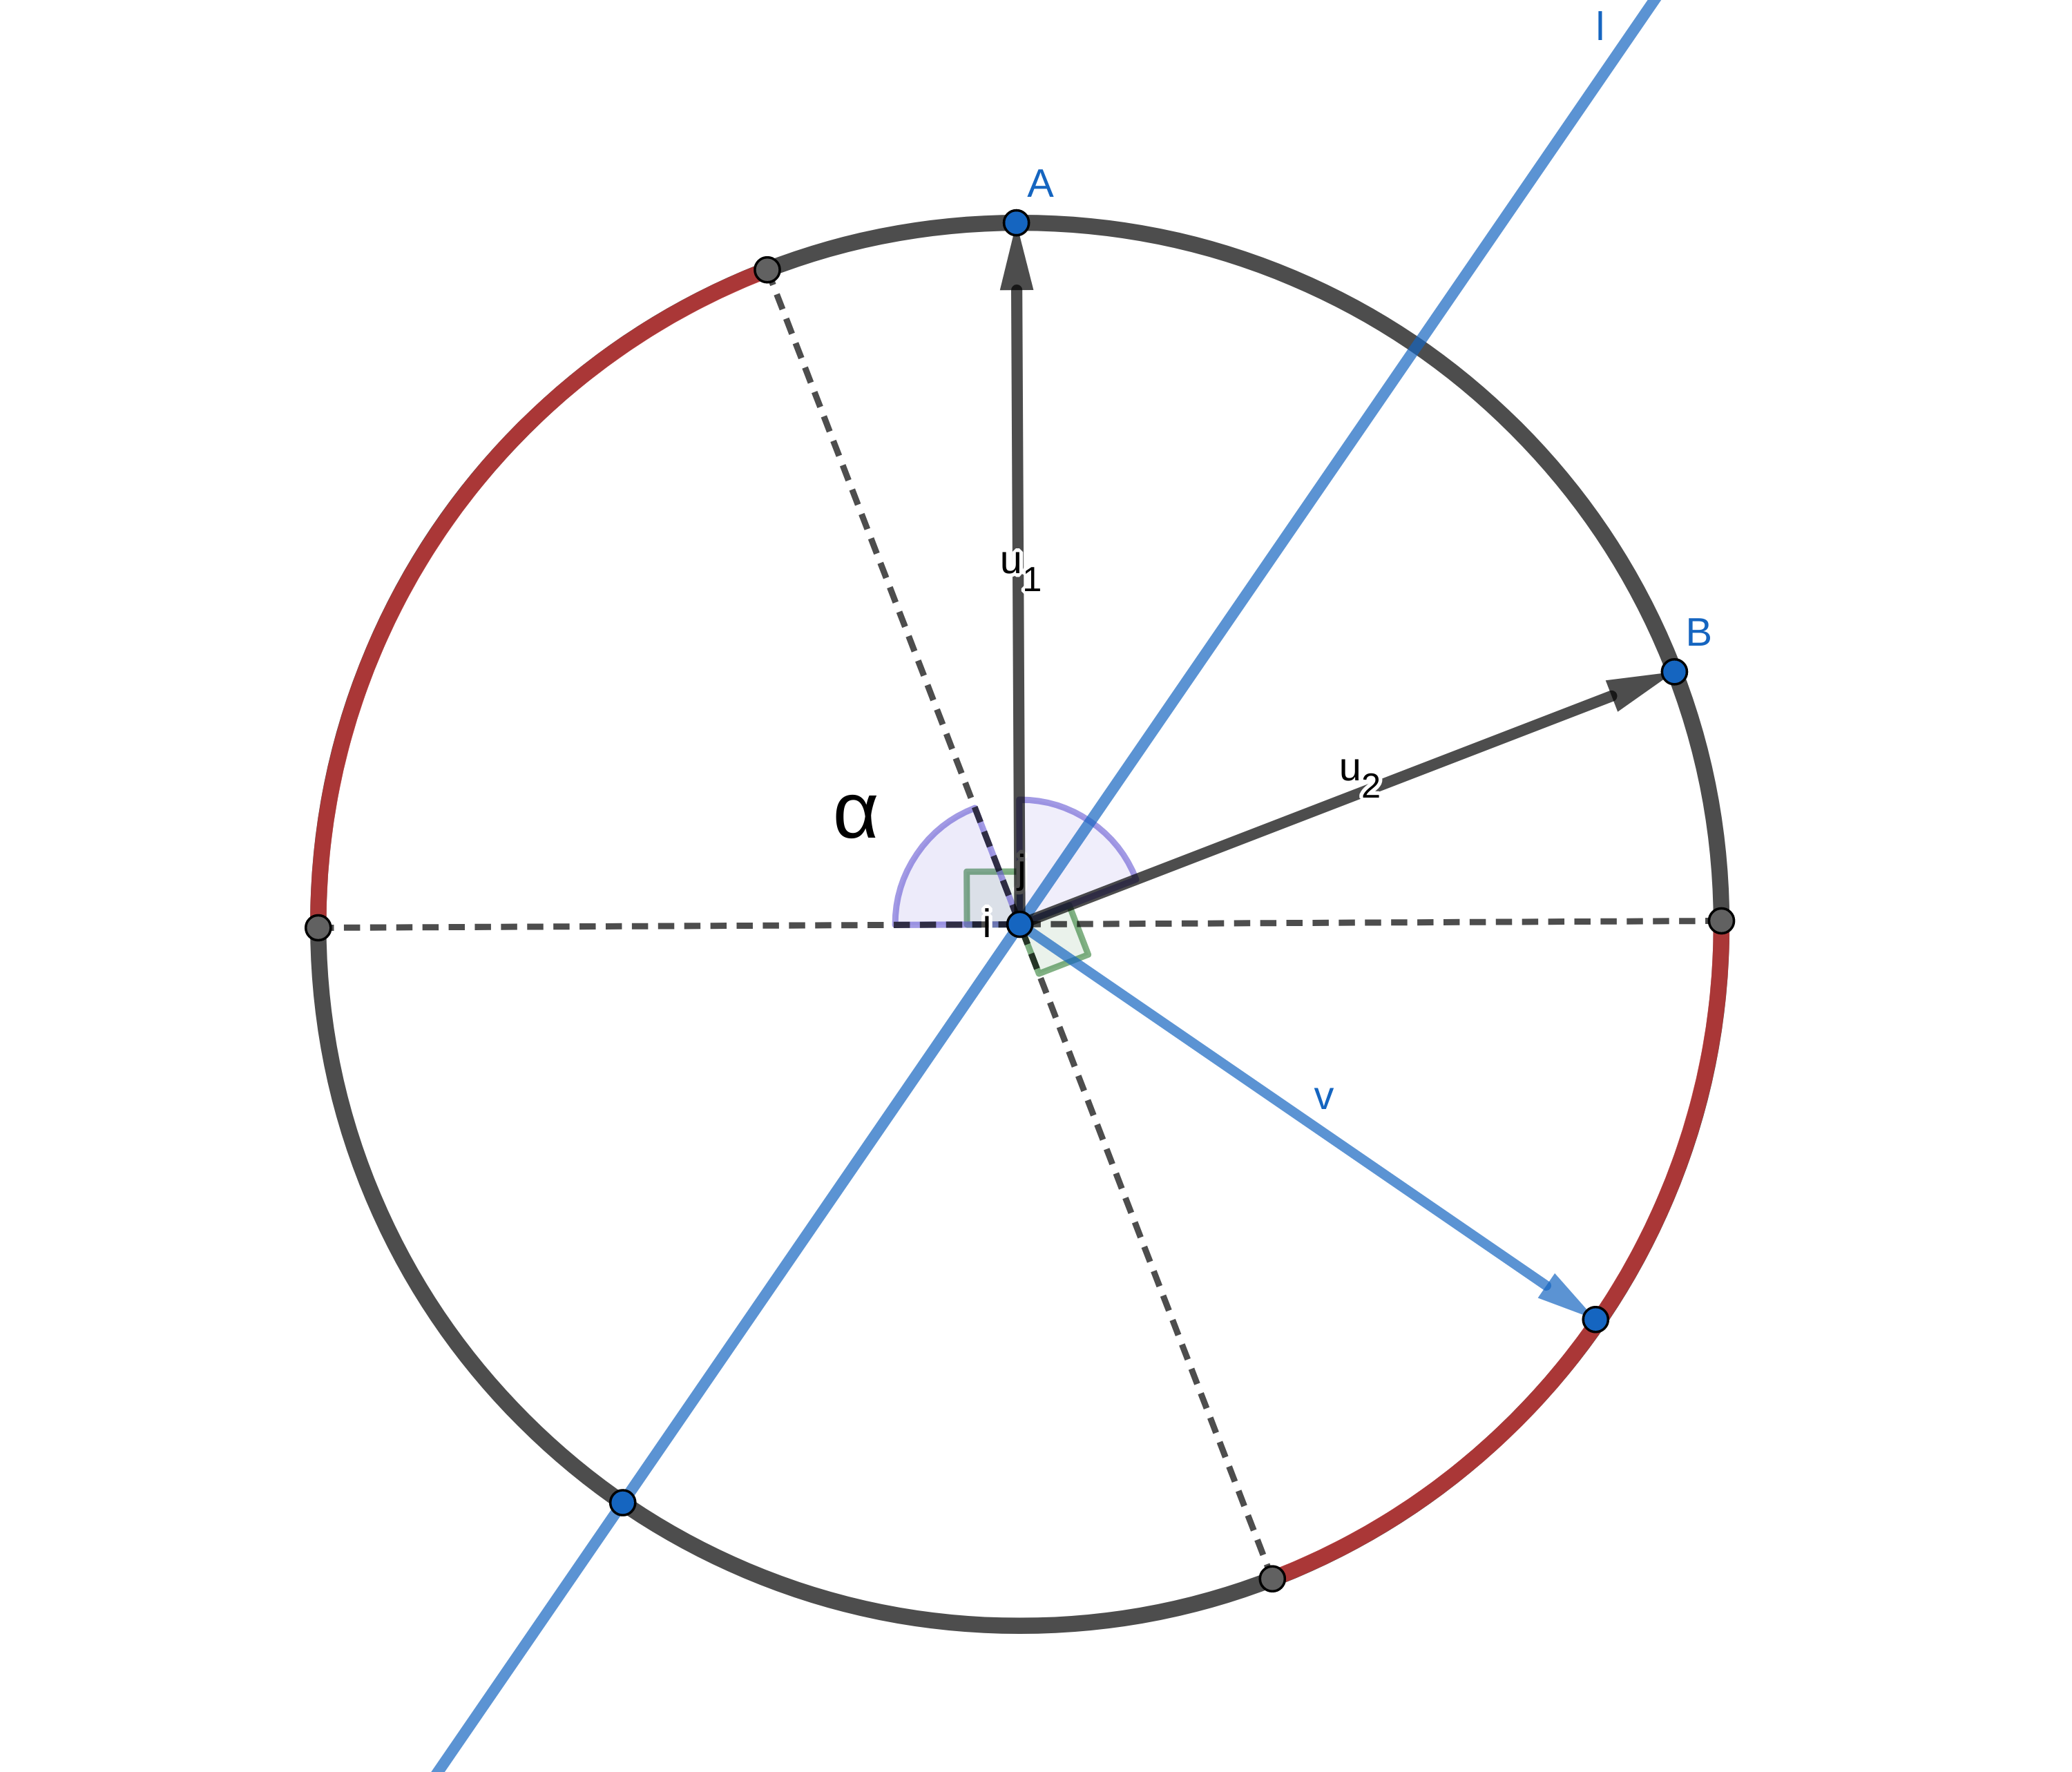
\includegraphics[width=0.8\textwidth]{images/Lemma.png}
\caption[width=0.8\textwidth]{Иллюстрация леммы для двумерного случая. Для разделимости исходных векторов необходимо и достаточно того, чтобы нормаль к гиперплоскости лежала в отмеченных красным секторах. Вероятность попасть в такие секторы равна $\frac{2\alpha}{2\pi} = \frac{\alpha}{\pi}$, но углы, отмеченные фиолетовым равны(как углы между перпеникулярами -- школьный факт), что и требовалось.}
\label{fig:fig2}
\end{figure}

\textbf{Лемма:}
$$\mathbb{P}(sign(v^Tu_i) \ne sign(v^Tu_j)) = \frac{\angle (u_i, u_j)}{\pi} = \frac{\arccos(u_i^T u_j)}{\pi}$$

\textbf{Доказательство:}
Проще говоря, хочется доказать, что вероятность отделить друг от друга два вектора случайной гиперплоскостью пропорциональна углу между этими векторами. Из симметрии сферы:
$$\mathbb{P}(sign(v^Tu_i) \ne sign(v^Tu_j)) = 2\mathbb{P}(v^Tu_i \geqslant 0, v^Tu_j < 0)$$
Событие из правой части образовано пересечением двух полупространств, угол между которыми как раз равен углу между векторами $u_i$ и $u_j$(обозначим его $\theta$), поэтому и вероятность такого события есть $\frac{\theta}{2\pi}$. Это доказывает первое равенство, а второе же получается выражение значения угла $\theta$ через $\arccos$. \\
\null \hfill \square

Итого:
$$ \Expect_v (C) = \frac{1}{2} \sum_{i = 1}^{n} \sum_{j=1}^{n} w_{ij} \frac{\arccos(u_i, u_j)}{\pi} = \frac{1}{2} \sum_{i = 1}^{n} \sum_{j=1}^{n} w_{ij} \frac{2\arccos(u_i, u_j)}{\pi(1 - u_i^T u_j)} \frac{1 - u_i^T u_j}{1} $$
Из ограничений SDP задачи, по которой получена матрица $Y$, получаем, что $|u_i| = 1$, значит $|u_i^T u_j| \leqslant 1$, причем выражение под модулем равно единице тогда и только тогда, когда $u_i = u_j$. Поэтому имеет смысл рассмотреть поведение функции $\frac{2 \arccos (x)}{\pi (1 - x)}$ на промежутке $[-1, 1)$. Оказывается, она \textbf{ограничена снизу} на этом промежутке константой $\alpha_{GW} \approx 0.878$, что можно, например, пронаблюдать на построенном графике.

\begin{figure}[h]
\centering
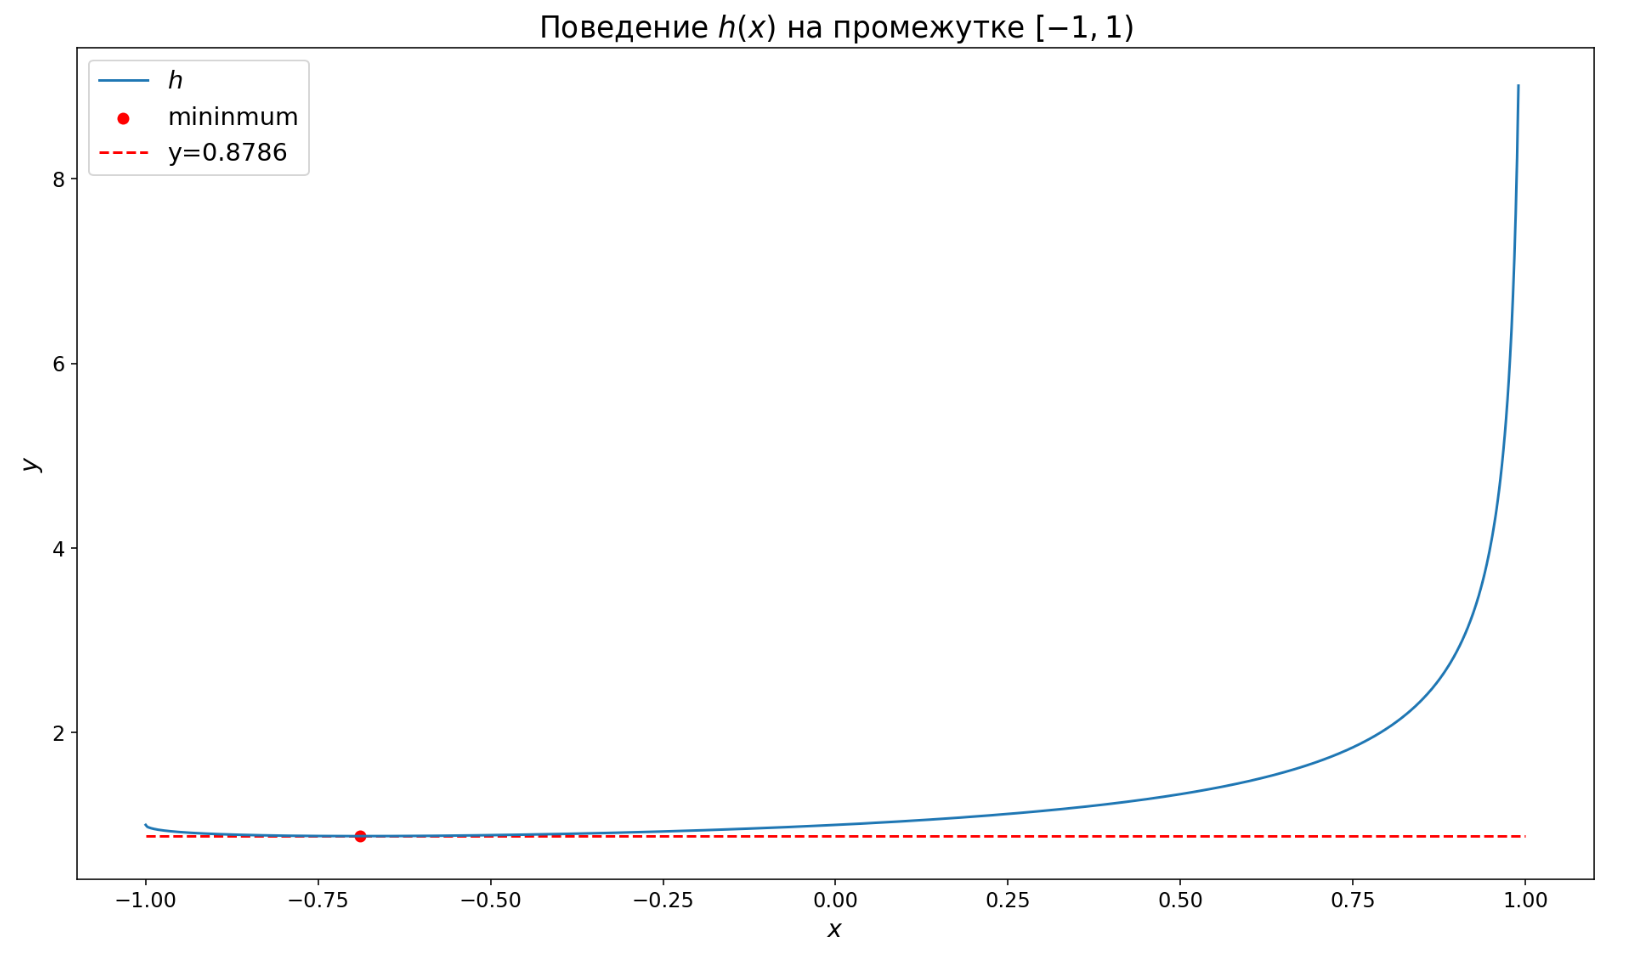
\includegraphics[width=0.8\textwidth]{images/h.png}
\caption[width=0.8\textwidth]{График функции $h(x)$}
\label{fig:fig3}
\end{figure}

Тогда
$$ \Expect_v (C) \geqslant \alpha_{GW} \frac{1}{4} \sum_{i = 1}^{n} \sum_{j=1}^{n} w_{ij} (1 - u_i^T u_j) = \alpha_{GW} p^* \geqslant \alpha_{GW} c^*$$
Т.к. любой ответ выданный алгоритмом будет не лушче чем оптимальный $c^*$, то и их среднее $\Expect_v (C)$ -- тоже. Значит
$$c^* \geqslant \Expect_v (C) \geqslant \alpha_{GW} \geqslant \alpha_{GW} p^* \geqslant \alpha_{GW} c^*$$
Утверждение доказано.\\
\null \hfill \square

\section{Эксперимент}

Реализовать описанный выше алгоритм можно с помощью общедоступных пакетов оптимизизации. Таким как раз является популярный пакет \href{https://cvxopt.org}{CVX} для Python3. Все материалы этого проекта, в том числе реализация и результаты тестирования доступны на моем \href{https://github.com/rvg77/max-cut}{Github}.

Стоит отметить, что в отличие от оригинальной статьи, моя реализация \textbf{повторяет} \textbf{несколько раз} случайную генерацию векторов на сфере и соответствующего разреза, чтобы по полученному набору ответов взять \text{среднее и максимум}. Так как количество таких повторов является не слишком большой константой(я взял $30$ для того, чтобы выборочное среднее хорошо приближало теоретический матож), а каждая такая итерация выполняется не слишком долго(из тяжелых операций там происходит только генерация случайного вектора и перемножение матрицы на вектор), то общее время работы возрастет на величину, которой можно принебречь. Оно и логично, внутри cvx наверняка используется что-то уж явно не легче чем перемножение матриц.

Также, мною было реализовано brute force решение экспоненциальной сложности, подсчитывающее точный ответ.\\

\subsection{План эксперимента}

\begin{enumerate}
    \item Зафиксируем несколько типов графов, из которых будем генерировать тест-сеты, а также количество графов в каждом тест сете $m=50$. Для каждого из типов графов будет по два тест-сета, которые будут отличаться количество вершин в графах, в данном случае это $n=10,20$.
    \item Сгенерируем графы для каждого из тест-сетов.
    \item Запустим на вообще всех графах brute force решение и SDP + алгоритм Гёманса-Уильямсона. Получим соответственно точный ответ, среднее по попыткам и максимум по по пыткам алгоритма для \textbf{каждого графа}.
    \item Проверим выполнимость теоретического утверждения для среднемго и исследуем насколько эффективным будет модификация с выбором максимума.
\end{enumerate}

\subsection{Исследуемые статистики}

\begin{enumerate}
    \item Посчитаем долю средних которые попадут в отрезок $[\alpha_{GW} c^*, c^*]$, где $\alpha_{GW} \approx 0.878$.
    \item Построим гистограмму для значения максимума из алгоритма поделить на точный ответ.
\end{enumerate}

\subsection{Описание наборов тестов}

Для тестирования были выбраны следующие стохастические типы графов(по два тест-сета на каждый в зависимости от количества вершин -- $10$ и $20$):

\begin{enumerate}
    \item Случайные 3-регулярные и 8-регулярные графы.
    \item Графы в модели Эрдёша — Реньи с $p=\frac{1}{2}, \frac{1}{4}, \frac{3}{4}$.
    \item Графы в модели Альберта-Барабаши со степенью $4$ и $\frac{n}{2}$.
    \item Графы, построенные по алгоритму Holm-Kim \cite{Holm}.
\end{enumerate}

\subsection{Анализ результатов}
Приведем сначала визуализации полученных результатов:

\begin{figure}[h]
\centering
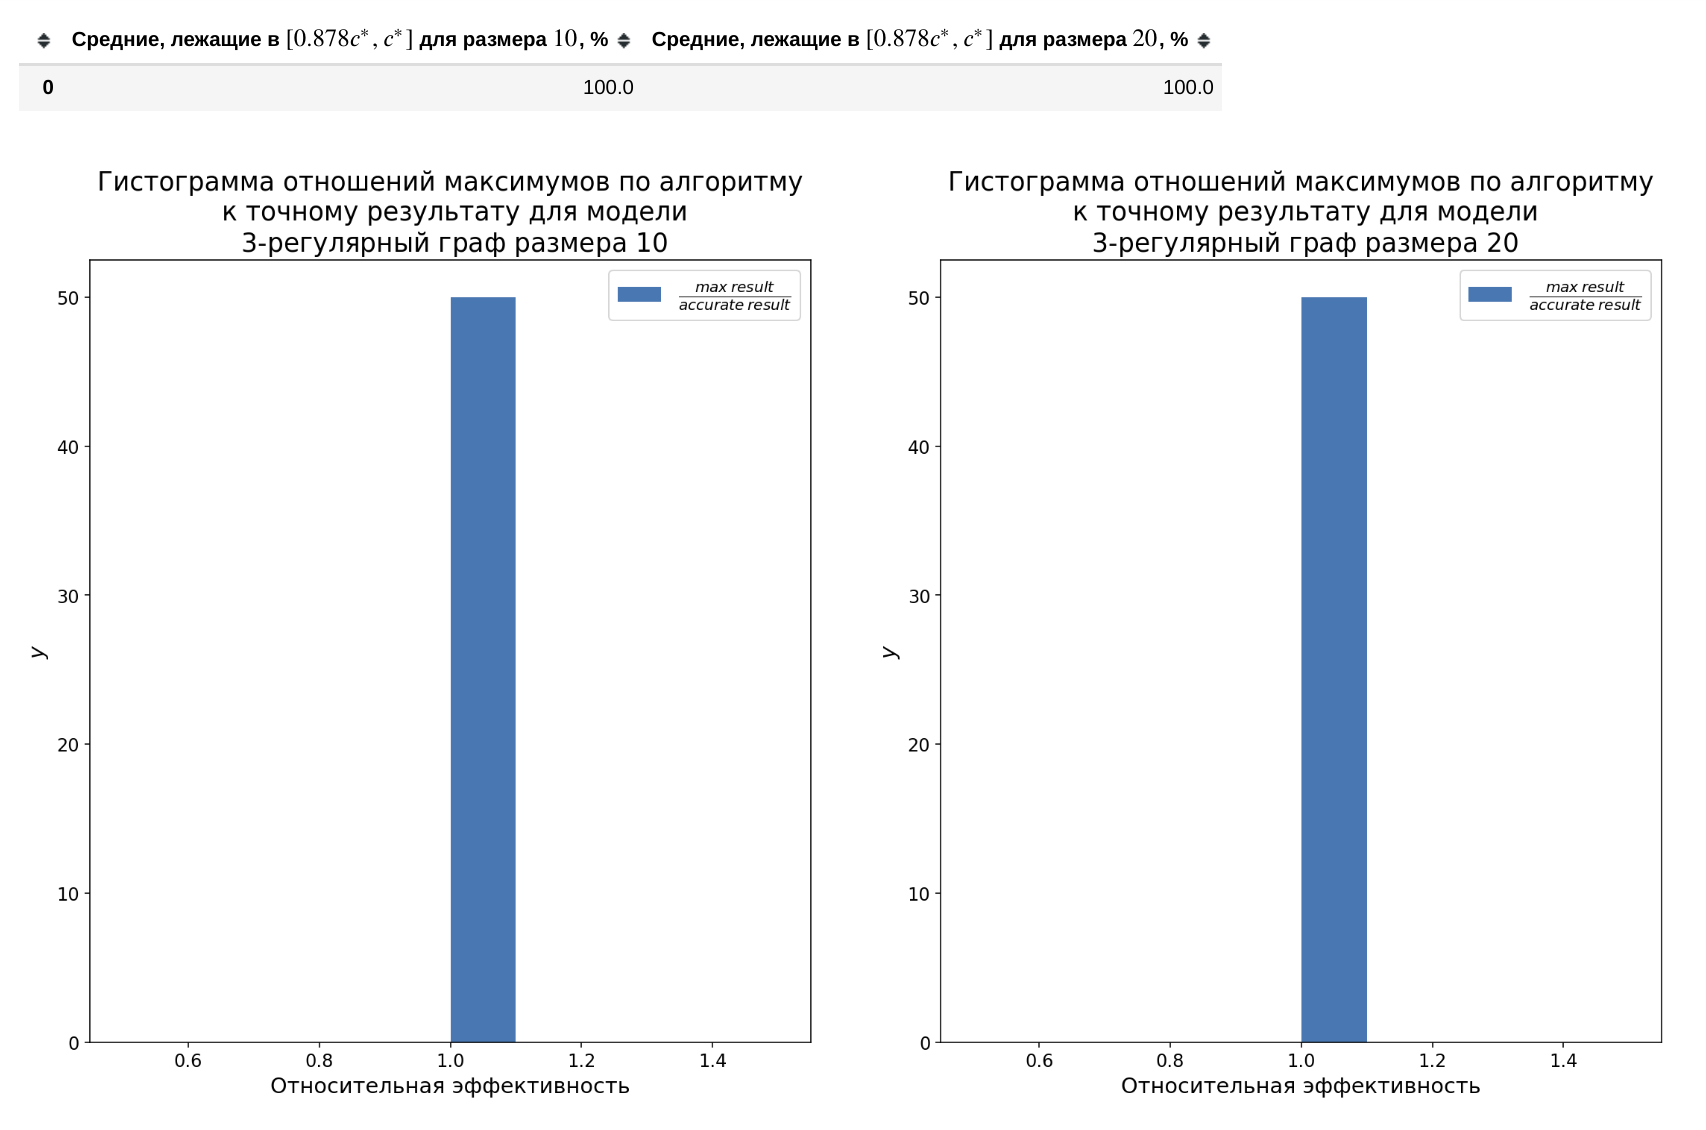
\includegraphics[width=1\textwidth]{images/1.png}
\caption[width=1\textwidth]{}
\label{fig:fig4}
\end{figure}

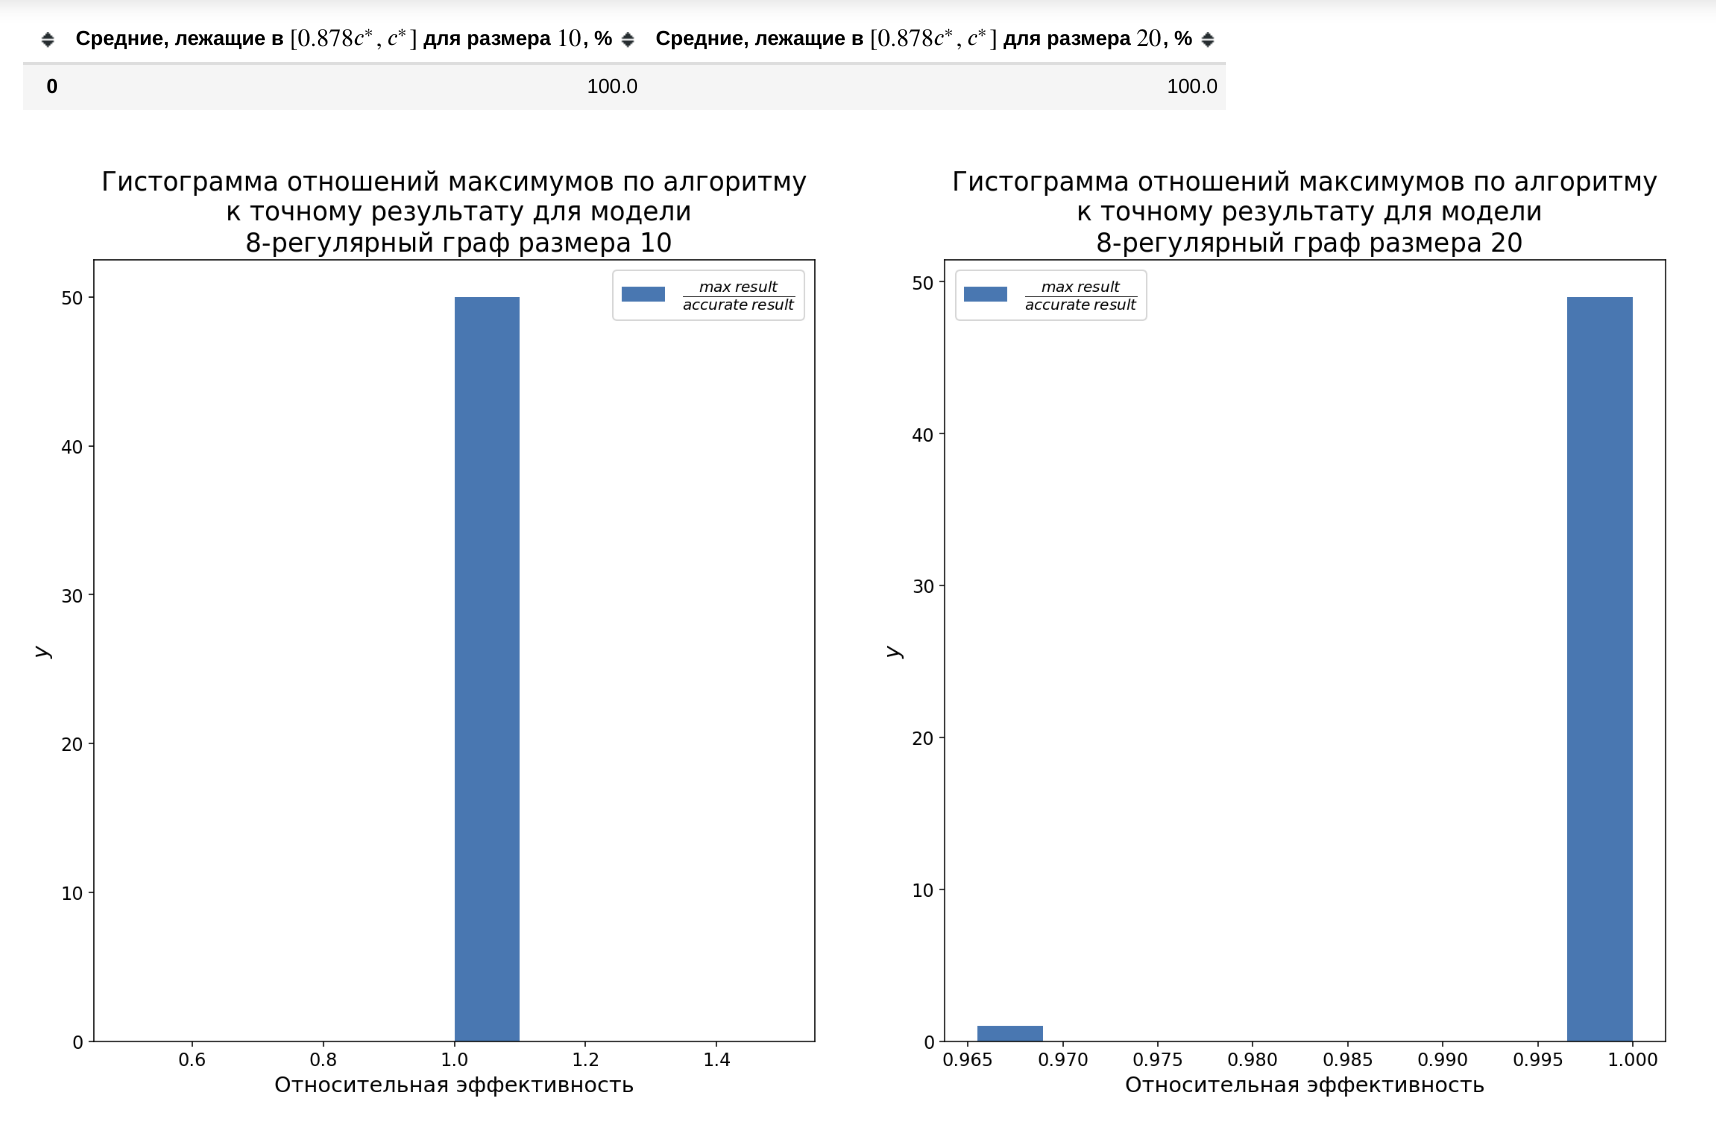
\includegraphics[width=1\textwidth]{images/2.png}

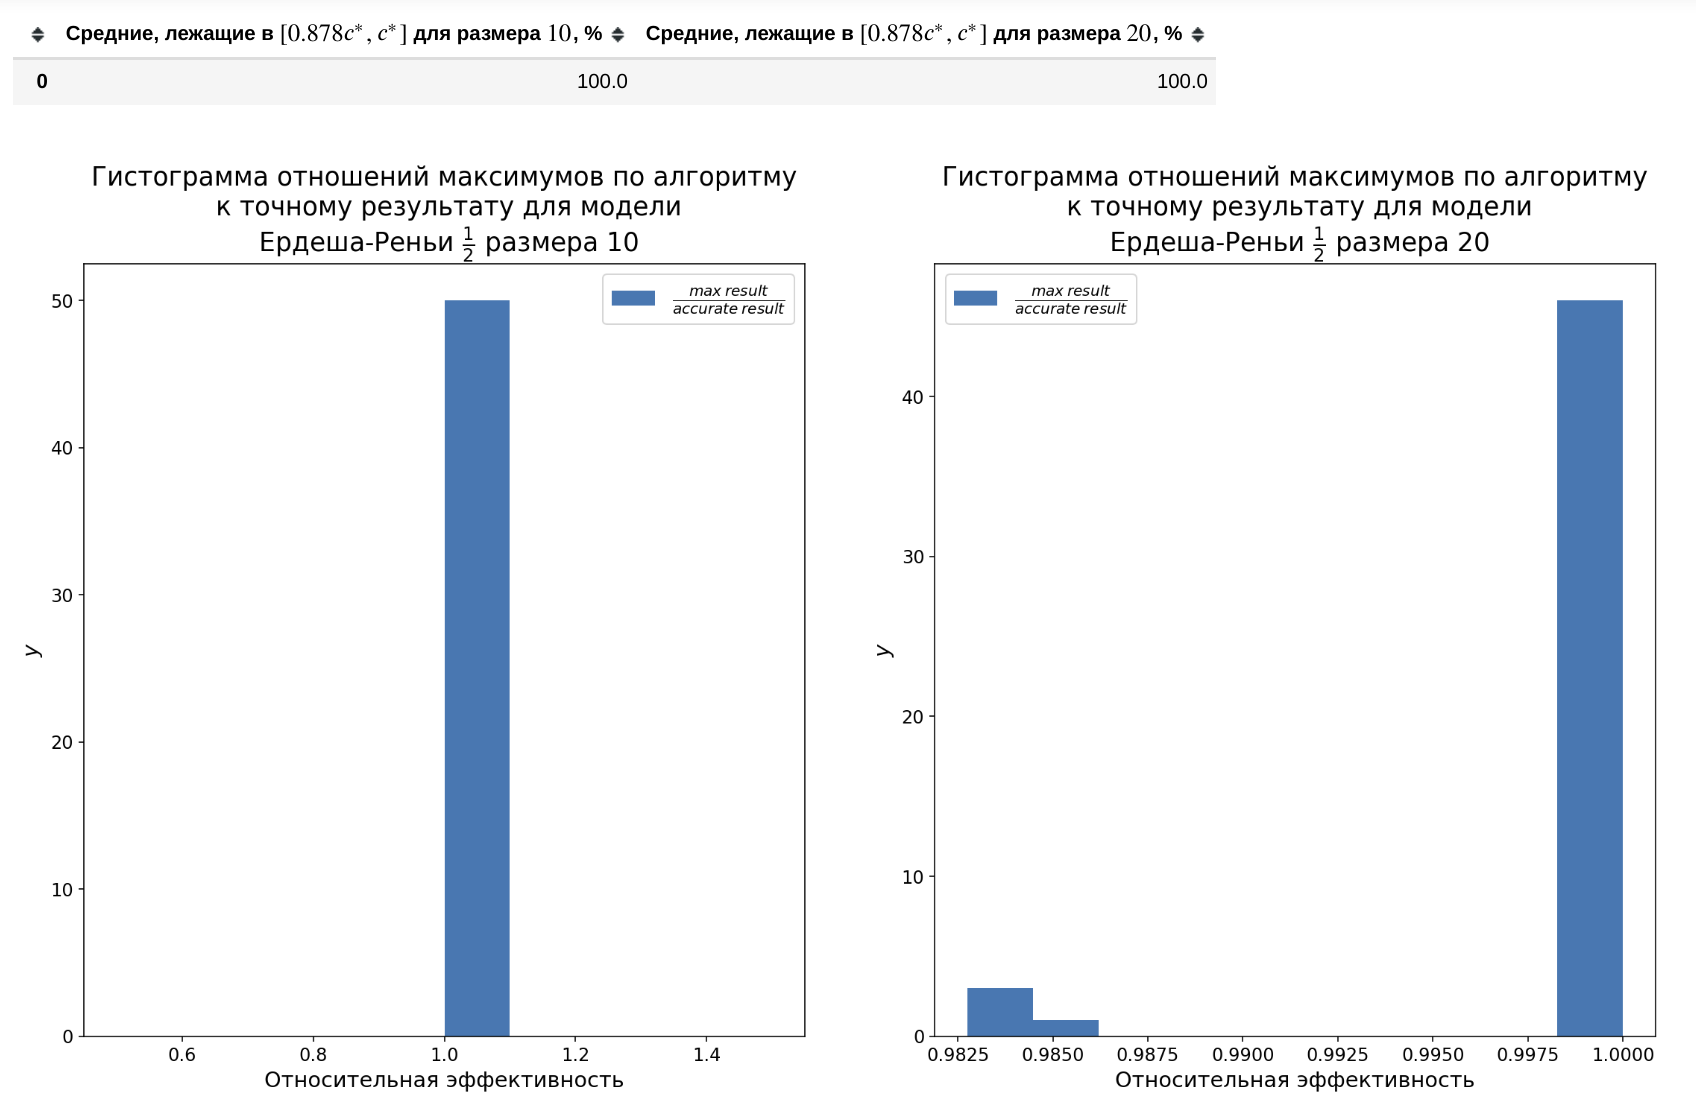
\includegraphics[width=1\textwidth]{images/3.png}

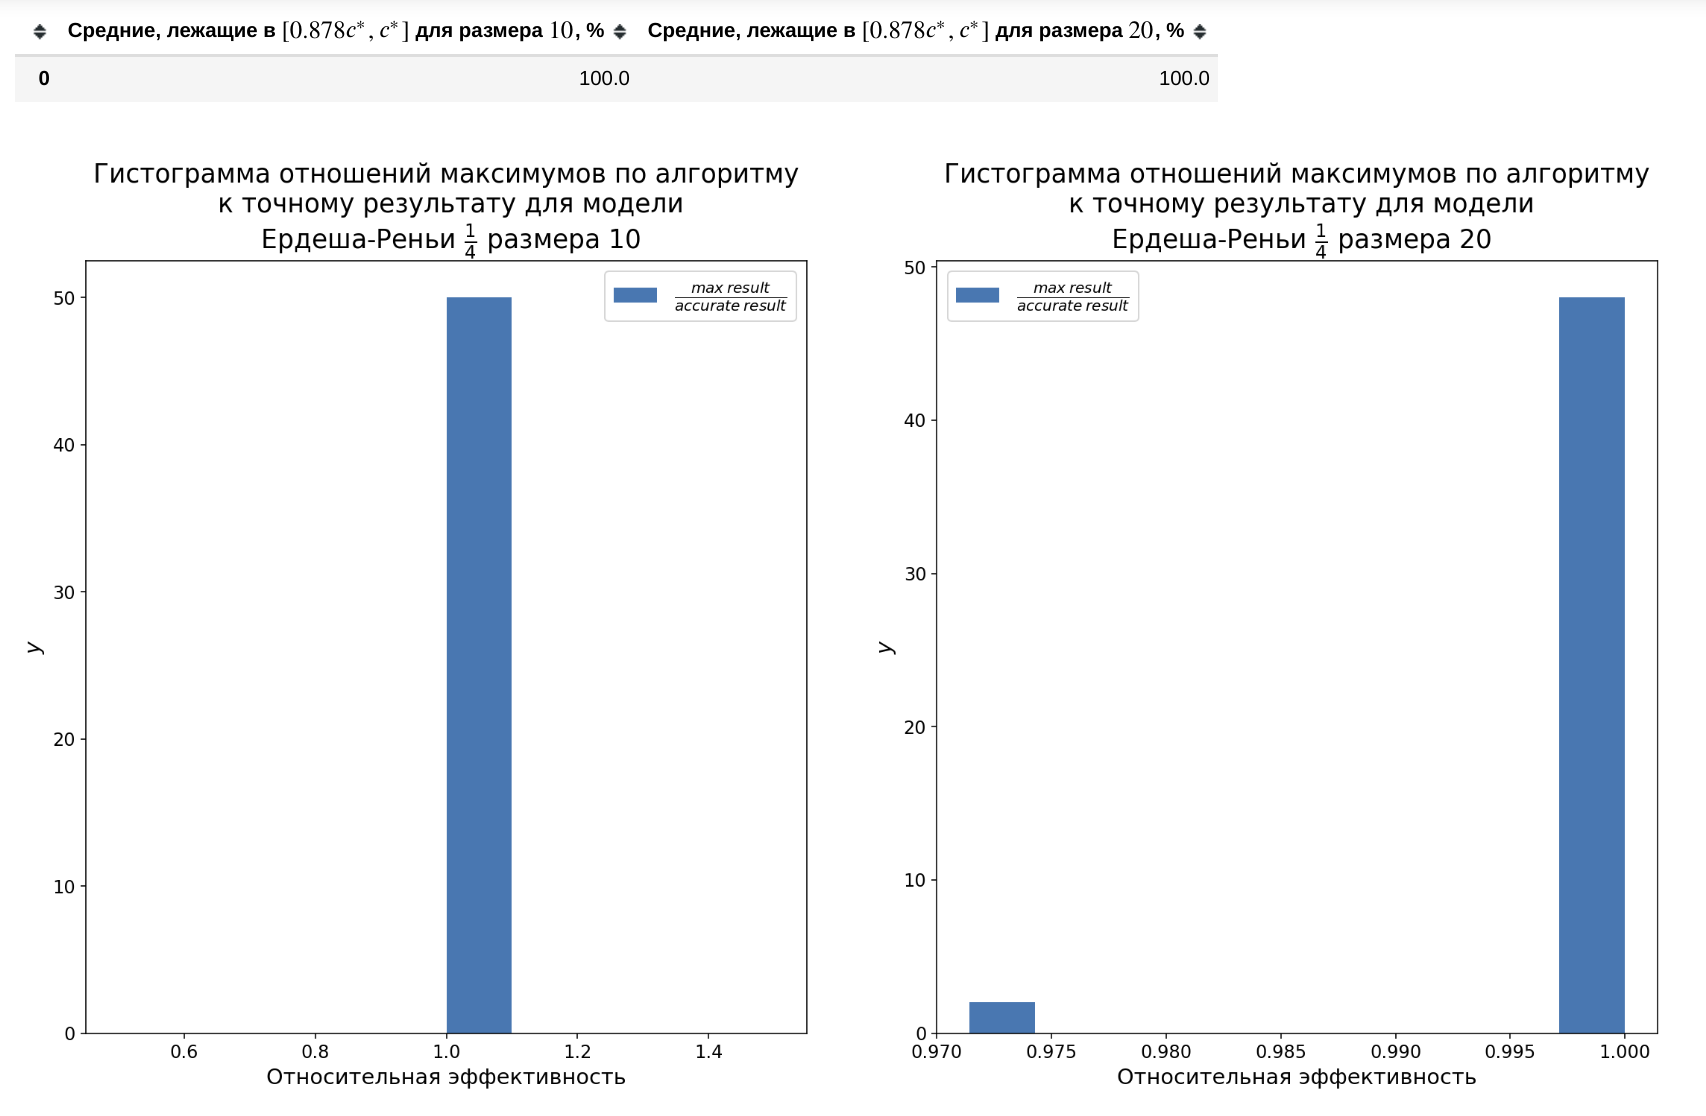
\includegraphics[width=1\textwidth]{images/4.png}

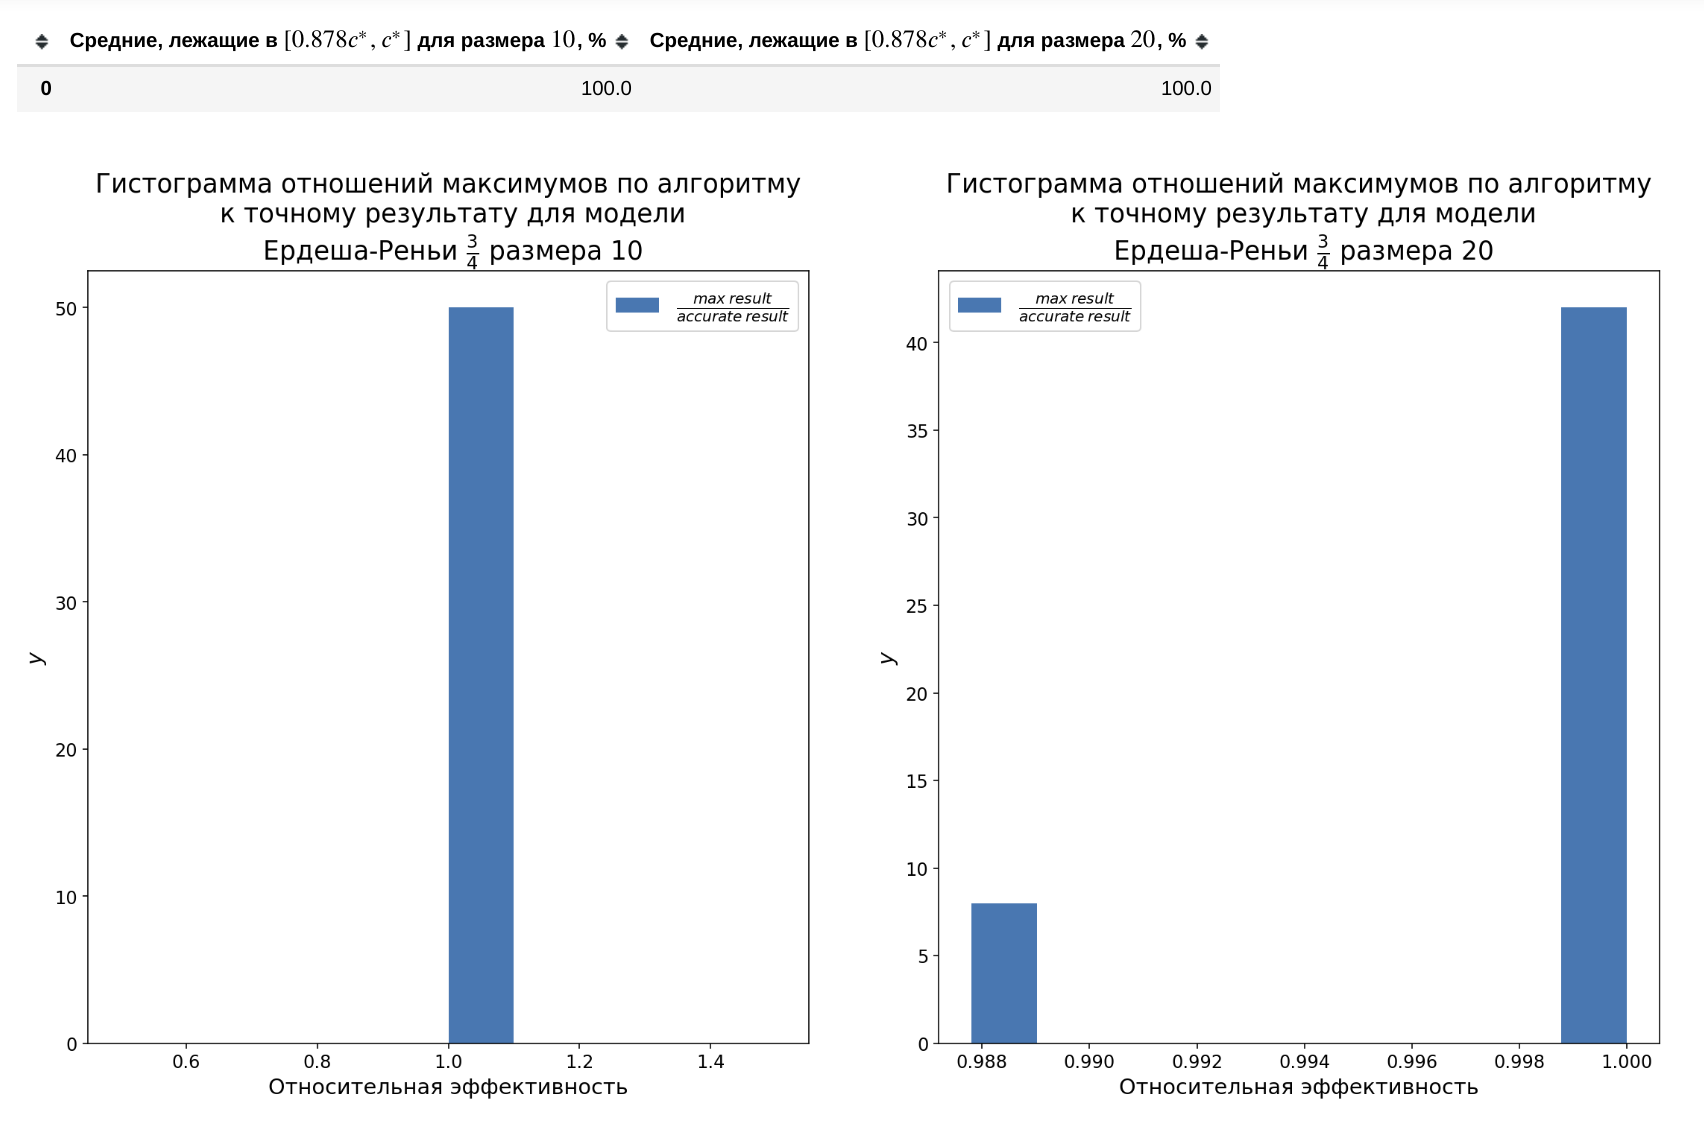
\includegraphics[width=1\textwidth]{images/5.png}

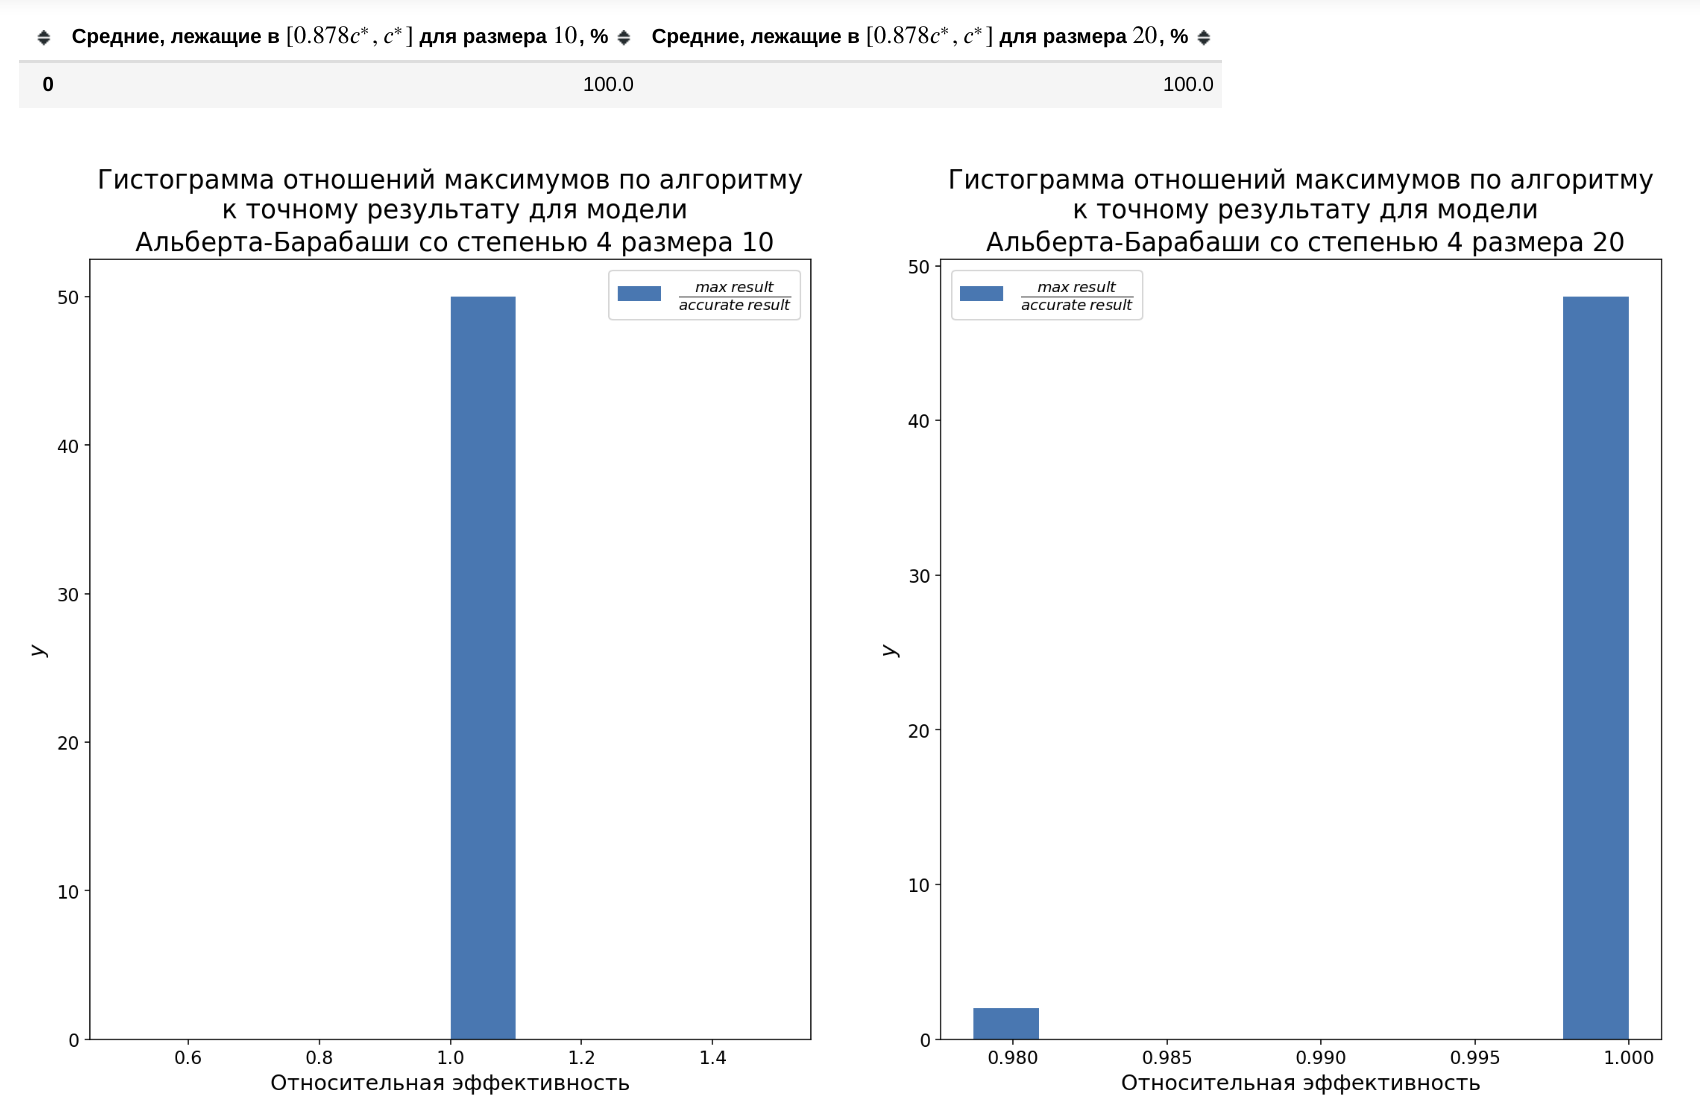
\includegraphics[width=\textwidth]{images/6.png}

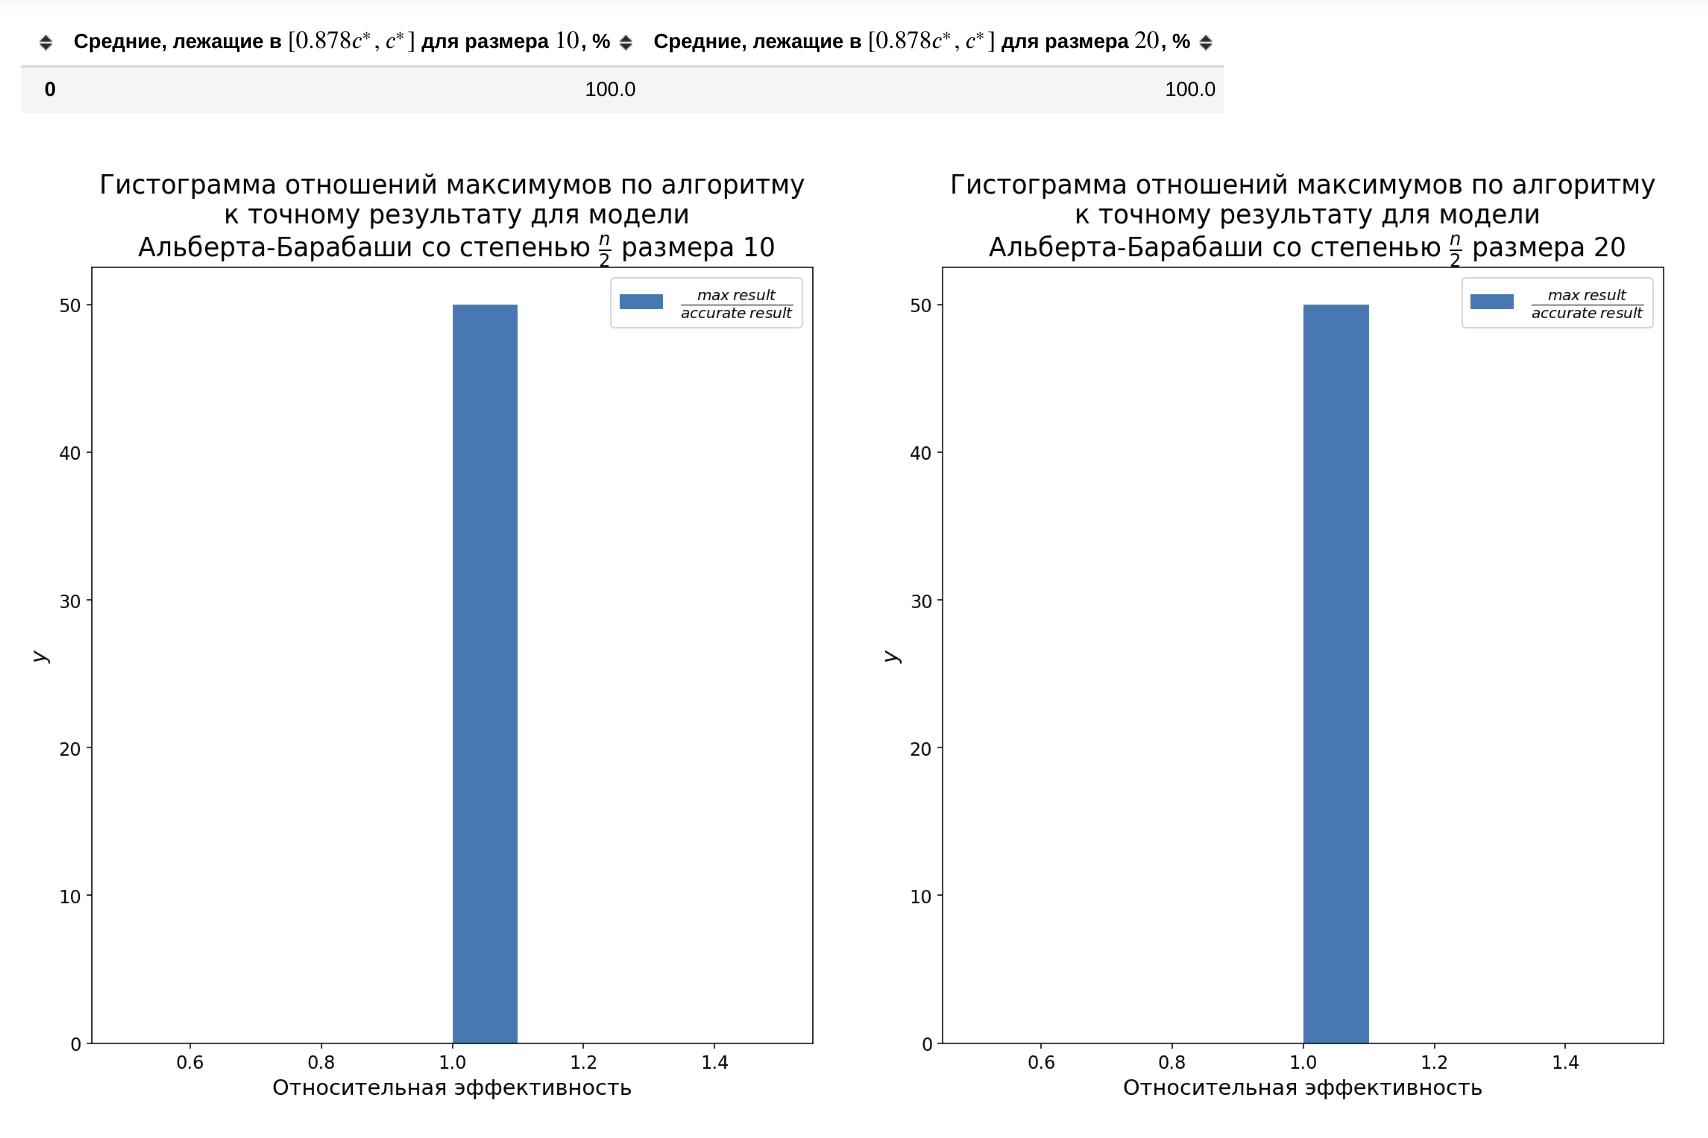
\includegraphics[width=1\textwidth]{images/7.png}

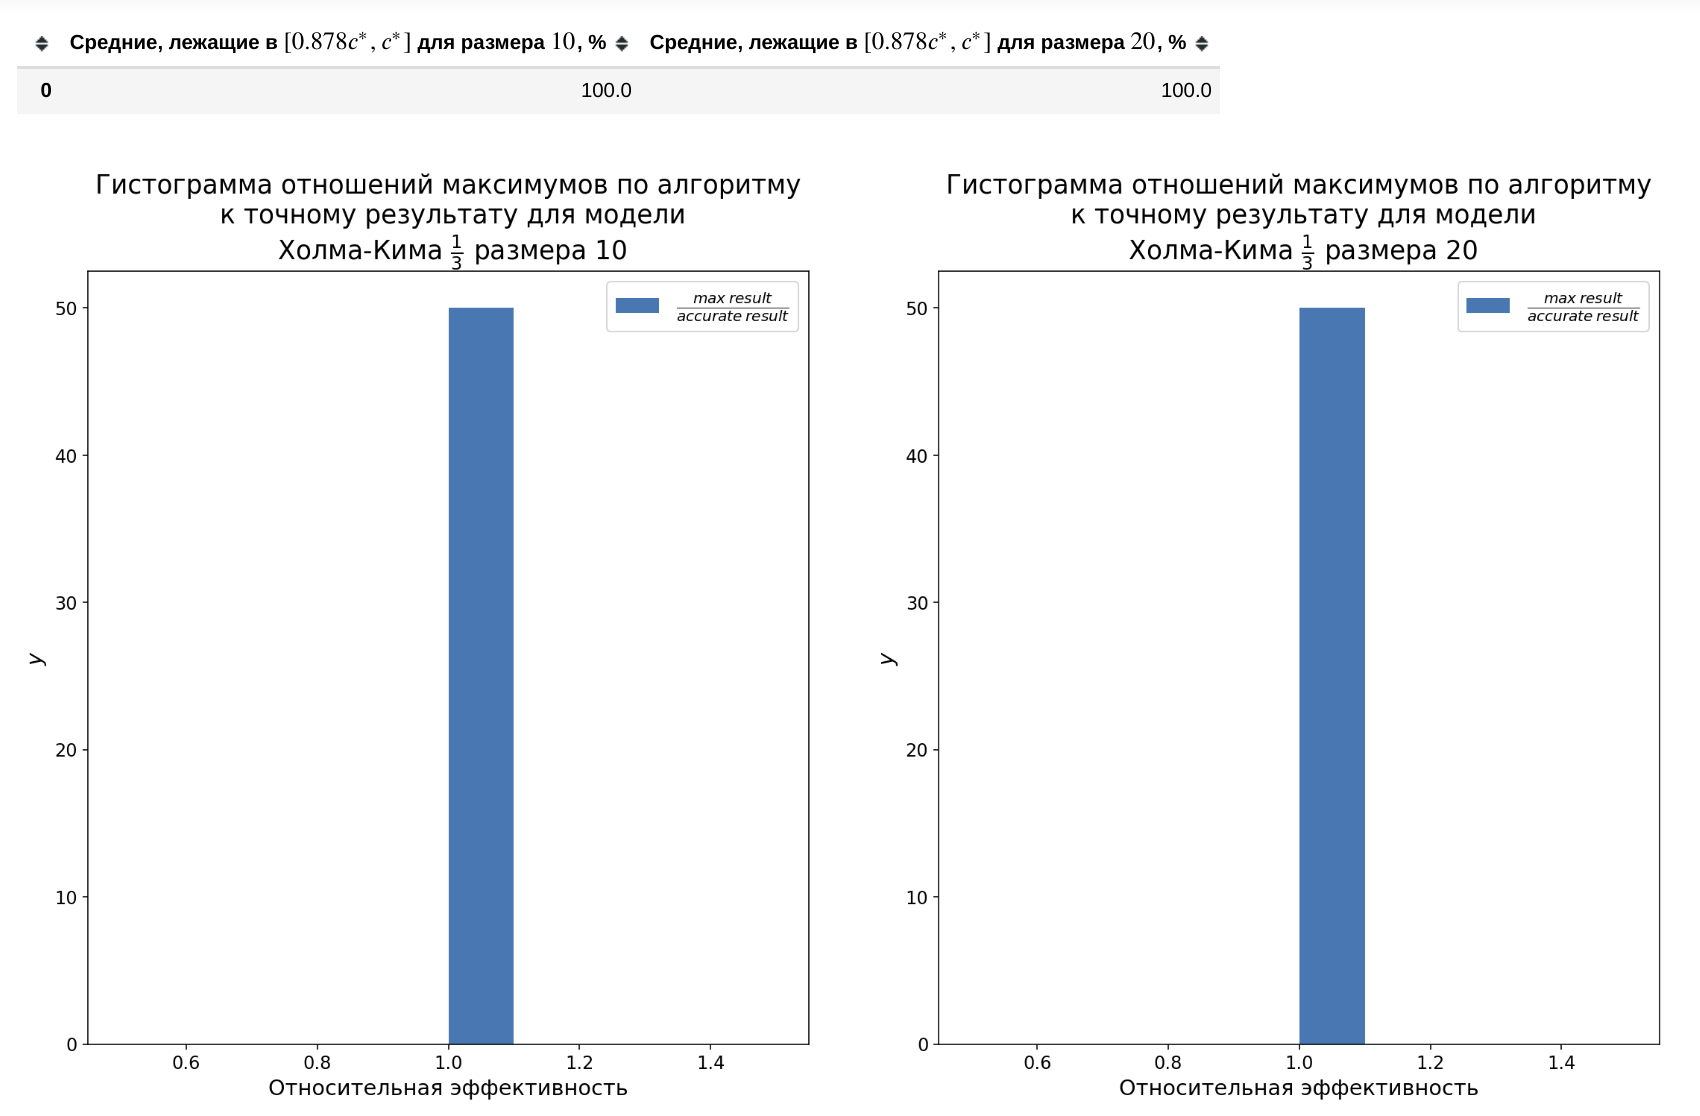
\includegraphics[width=1\textwidth]{images/8.png}

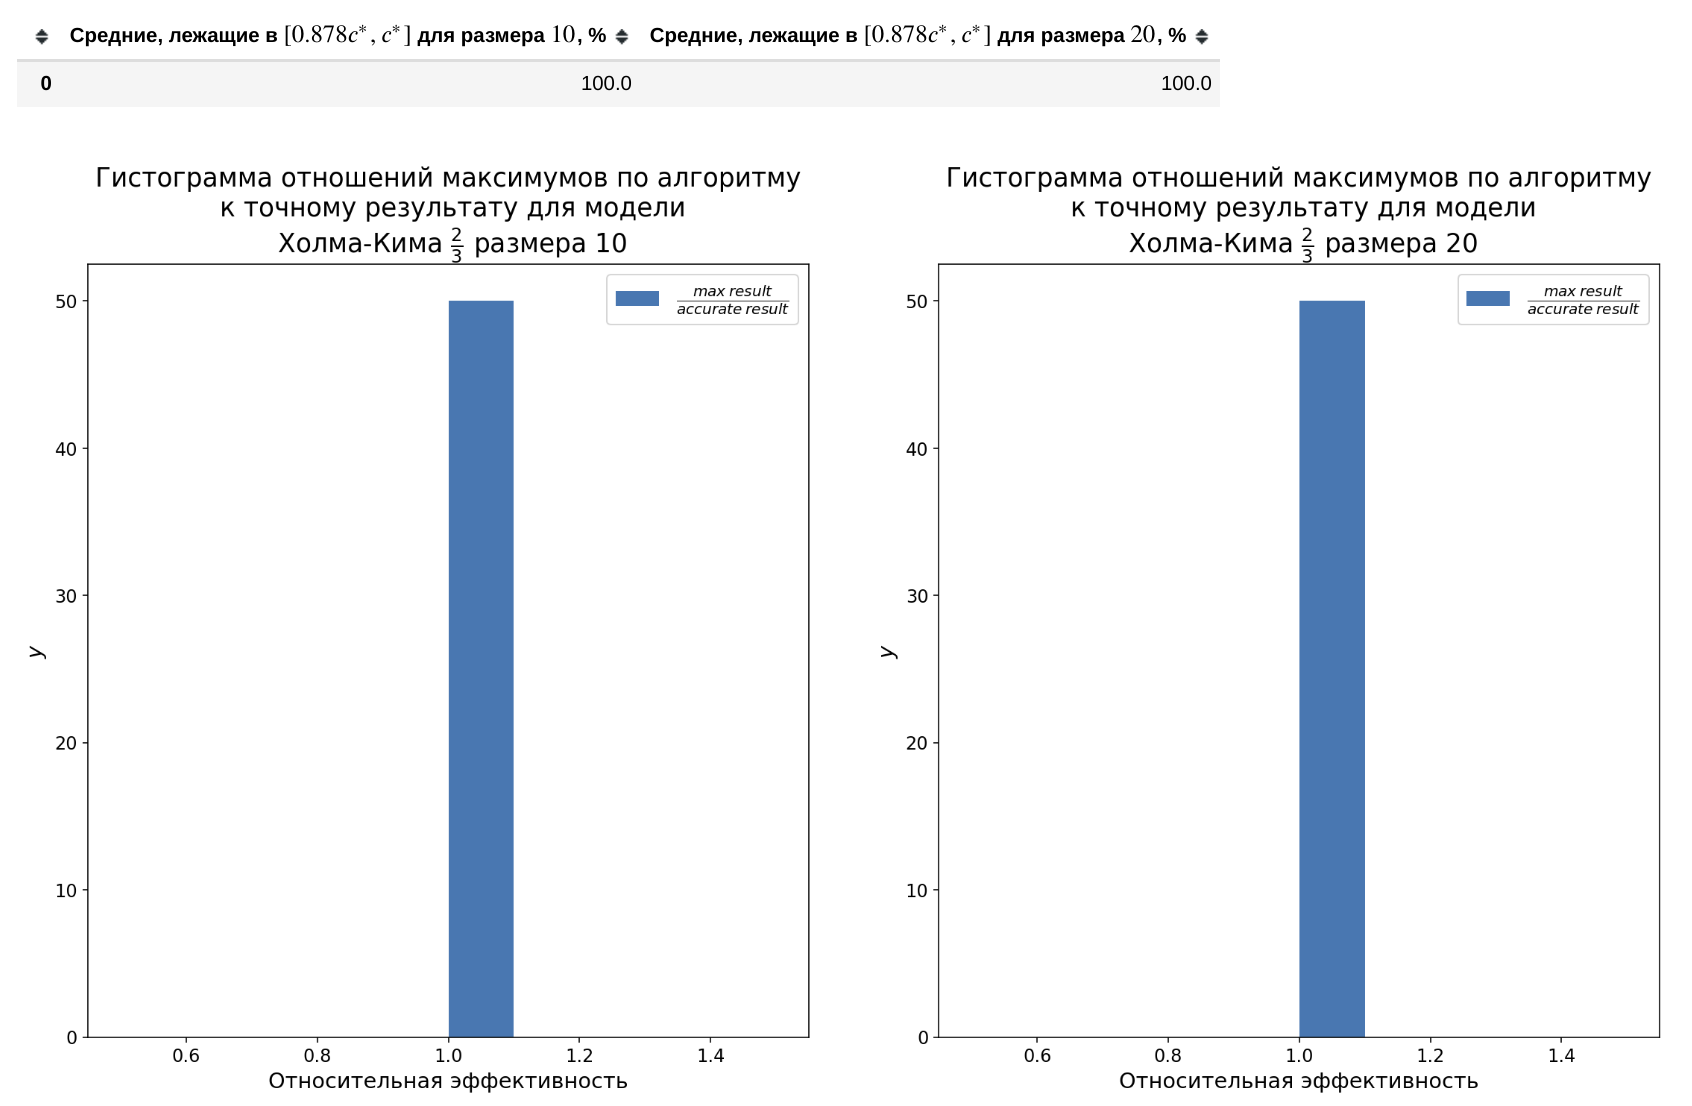
\includegraphics[width=1\textwidth]{images/9.png}

\begin{enumerate}
    \item Как видим, доказанное теоретически утверждение согласуется со всем полученными результатами.
    \item На данных размерах графов и при всех рассмотренных их стохастических типах идея, брать из всех результатов максимум, отлично себя показала и дает точный реультат в более чем $80\%$ случаев.
    \item На затраты по памяти не стоит обращать внимание, потому что при данных размерах графа они близки к нулю.
    \item Что касается времени, то на рассматриваемых тестовых данных переборное решение требует порядка $20$ секунд в среднем на один граф, в то время как SDP решение требует порядка времени порядка $1$ секунды.
\end{enumerate}

\section{Заключение}
Подводя итоги, можно сказать, что в течение выполнения проекта удалось ознакомиться с алгоритмом Гёманса-Уильямсона, вопроизвести его доказательство, реализовать его, добавив, хоть и несложную, но всё-таки модификацию, а также протестировать его на тест-сетах разнообразных типов случайных графов. Результаты эксперимента согласуются с теоретически доказанныи фактами, а модификация показывает результаты с приемлимым уровнем точности, хотя стоит отметить, что для более тщатательного исследования необходимо значительно увеличить размеры графов, что требует огромных вычислительных мощностей, которыми я, к сожалению, не обладаю.

\begin{thebibliography}{9}

\bibitem{reduction} 
David Steurer: Reduction from 3 SAT to MAX CUT,\\
\url{http://www.cs.cornell.edu/courses/cs4820/2014sp/notes/reduction-maxcut.pdf}

\bibitem{Holm}
P. Holm and B. J. Kim: “Growing scale-free networks with tunable clustering”, Phys. Rev. E, 65, 026107, 2002.\\
\url{https://networkx.github.io/documentation/networkx-1.9.1/reference/generated/networkx.generators.random_graphs.barabasi_albert_graph.html}

\end{thebibliography}

\end{document}
